\documentclass[10pt]{article}   	% use "amsart" instead of "article" for AMSLaTeX format
\usepackage{geometry}                		% See geometry.pdf to learn the layout options. There are lots.
\usepackage[english]{babel}
\geometry{a4paper}                   		% ... or a4paper or a5paper or ... 
%\geometry{landscape}                		% Activate for for rotated page geometry
%\usepackage[parfill]{parskip}    		% Activate to begin paragraphs with an empty line rather than an indent
\usepackage{graphicx}				% Use pdf, png, jpg, or epsß with pdflatex; use eps in DVI mode
\usepackage{fontspec}
\usepackage{multicol}
\setmainfont{Arial}
					
\linespread{1.1}			% TeX will automatically convert eps --> pdf in pdflatex		
\usepackage{amssymb}
\usepackage{eurosym}
\usepackage{colortbl}
\title{MorphicDraw}
\author{Stephan J.C. Eggermont, Sensus}
\begin{document}
\setlength{\parindent}{0pt}
\maketitle
\begin{quote}
\em
MorphicDraw is a drawing application demonstrating some of the power of Morphic.
Morphic is a powerful graphics environment, used in Self, Squeak, Cuis and Pharo.
In an iterative and incremental process we'll build up an application that supports
drawing connected figures.
\end{quote} 

\section{A Morphic Application}
\begin{figure}[htb]
\begin{center}
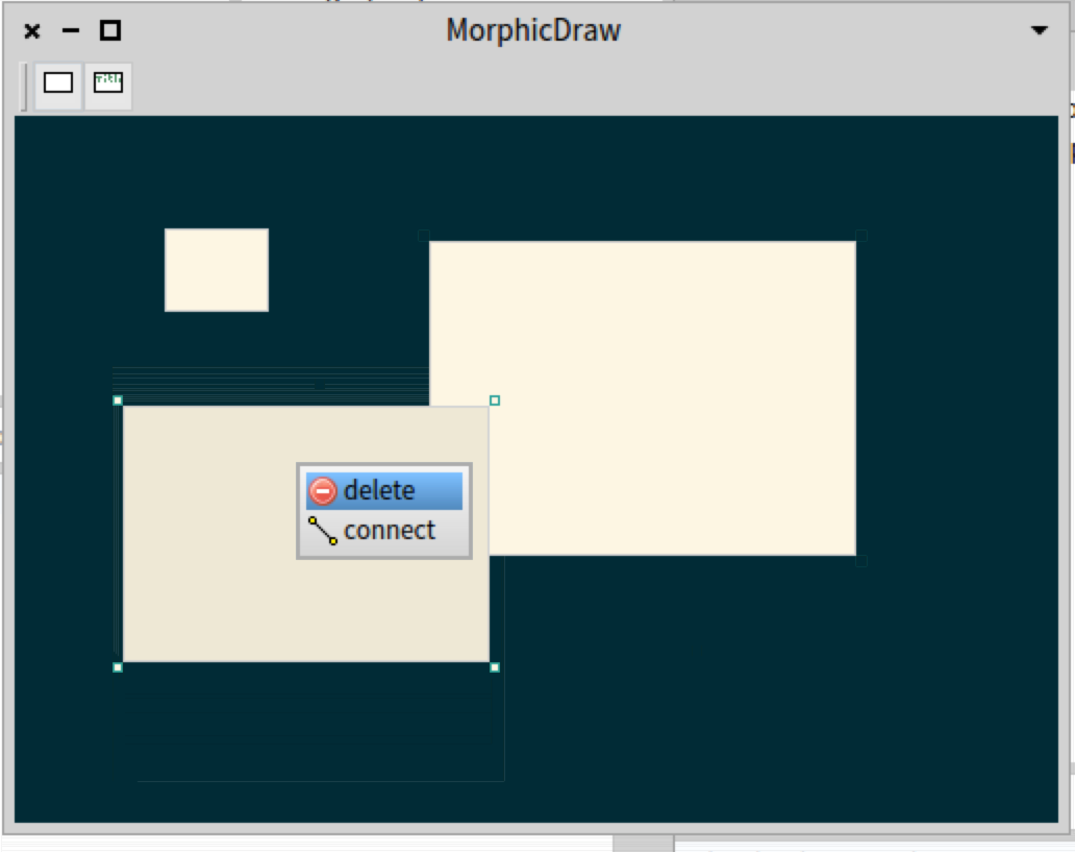
\includegraphics[width=200pt]{SimpleMorphicDrawWindow.pdf}
\caption{A first iteration of the main window of MorphicDraw}
\label{1stIteration}
\end{center}
\end{figure}
The first iteration (Figure \ref{1stIteration})  shows an application window 
with a toolbar and a drawing area. In the drawing area there are 
three graphical shapes, one of which is selected. A context menu
for the selected shape shows options to delete it and to connect it.

\subsection{An application with a window}
Add a class that represents the application. It has instance variables for 
the different parts. 

\begin{verbatim}
Object subclass: #MorphicDraw
    instanceVariableNames: 'window tools dock'
    classVariableNames: ''
    category: 'MorphicDraw-Model'
\end{verbatim}

Creating a window in Morphic is simple. Open a workspace and DoIt
\begin{verbatim}
StandardWindow new openInWorld 
\end{verbatim} 
This creates a window and opens it on the screen. 
It already has default behaviour for closing and resizing, and a default title. 
All graphical elements in Morphic are subclasses of Morph, and the 
World is a container for all of them. Opening a Morph in the world
positions it and makes it visible. An alternative to opening it directly is
to add it to the (mouse) cursor. In Morphic this is called the hand.
DoIt:
\begin{verbatim}
StandardWindow new openInHand 
\end{verbatim} 
The window is then positioned by clicking.

The MorphicDraw application uses the first, but needs to change 
the window title and default size.

\begin{verbatim}
MorphicDraw>>createWindow
    window := StandardWindow new
        setLabel: 'MorphicDraw';
        extent: 400@400;
        yourself.
\end{verbatim}

StandardWindow is part of PolyMorph. PolyMorph makes the 
Window responsible for adding predefined user interface widgets
to the application Window. For that it uses the TEasilyThemed 
trait. It adds a lot (163 in my current image) of convenience methods.

In Morphic, a toolbar in a window has buttons on it. This iteration of
MorphicDraw uses two buttons to be able to create two different 
graphical shapes.

\begin{verbatim}
MorphicDraw>>createNewCardButton
    ^ window
        newButtonFor: self
        getState: nil
        action: #newCard
        arguments: nil
        getEnabled: nil
        labelForm: MDIcons default cardIcon
        help: 'New Card' translated
\end{verbatim}
The help text is shown when hovering the mouse over the button.
The button is always enabled, and sends the \#newCard message 
without any arguments to self when it is pressed. It has no 
state-dependent behaviour or shape. The icon for the button
is provided by MDIcons default cardIcon.

The button for the other shape is similar:
\begin{verbatim}
MorphicDraw>>createNewRectangleButton
    ^ window
        newButtonFor: self
        getState: nil
        action: #newRectangle
        arguments: nil
        getEnabled: nil
        labelForm: MDIcons default rectangleIcon
        help: 'New Rectangle' translated
\end{verbatim}

A toolbar in Morphic consists of two parts, a ToolDockingBar and
a Toolbar. The Toolbar is added 

\begin{verbatim}
MorphicDraw>>createToolBar
    tools := window newToolbar: (Array with: self createNewRectangleButton with: self createNewCardButton).
    dock := window newToolDockingBar.
    dock addMorphBack: tools
\end{verbatim}

At the class side add a method to open the application

\begin{verbatim}
MorphicDraw>>open
    ^self new open
\end{verbatim}

\section{Shapes and PasteUpMorph}

\section{Toolbar}
\section{Connecting}



\section{Selection and resizing}



\end{document}  